% ------------------------------ %
%                                %
%    Preamble by Rasmus Wiuff    %
%        rwiuff@gmail.com        %
%                                %
% -------------------------------%

%Author(s), Course variables
\newcommand{\titl}{Implementering \& Test}
\newcommand{\handin}{Indsæt dato}
\newcommand{\authOne}{Rasmus Wiuff}
\newcommand{\authTwo}{Mathies Henriksen}
\newcommand{\authThree}{Max-Emil Scotten}
\newcommand{\authFour}{Kasper Sylvest}
\newcommand{\SIDOne}{s163977}
\newcommand{\SIDTwo}{s200747}
\newcommand{\SIDThree}{s204633}
\newcommand{\SIDFour}{s205281}
\newcommand{\courseno}{02161}
\newcommand{\course}{Software Engineering 1}
\newcommand{\lb}{\\}
%Basics
\documentclass[a4paper, danish]{article}
\usepackage[utf8]{inputenc}
\usepackage[T1]{fontenc}
\usepackage[bitstream-charter]{mathdesign}
% \usepackage{XCharter}
\usepackage{babel}
\usepackage[moderate]{savetrees}
%Symbols and scientifics
\usepackage{amsmath, bm}
\numberwithin{equation}{section}
\usepackage{physics}
\usepackage{mathtools}
\usepackage{siunitx}
\sisetup{
    per-mode = power ,
    round-mode = figures ,
    round-precision = 3 ,
    scientific-notation = false ,
    output-decimal-marker = {.} ,
    exponent-product = \times ,
    separate-uncertainty = true ,
    uncertainty-separator = \ ,
    range-phrase = - ,
    range-units =  single ,
    inter-unit-product = \ensuremath{{\cdot{}}} ,
    number-unit-product = \ ,
    multi-part-units = single ,
}

%Appendix, TOC and Bibliography
\usepackage{appendix}
\renewcommand\appendixtocname{Appendices}
\usepackage[nottoc]{tocbibind}
\setcounter{tocdepth}{2}
\usepackage{lastpage}

%Figures
\usepackage[svgnames]{xcolor} % Required to specify font color
\usepackage{float}
\usepackage{graphicx}
\usepackage{setspace}
\usepackage{subcaption}
\usepackage[format=plain,
    labelfont={bf,it,footnotesize},
    textfont={it,footnotesize}]{caption}
% \captionsetup[table]{name=Huskeord}
\captionsetup{font={stretch=0.9}}
\usepackage{wrapfig}
\usepackage[a4paper, centering, rmargin=2.5cm, tmargin=2.5cm, lmargin=2.5cm, bmargin=3.5cm]{geometry}
\usepackage{etoolbox}
\usepackage{verbatim}
\usepackage[space]{grffile}
\usepackage[final]{pdfpages}
\usepackage{array}
\usepackage{multirow}
\usepackage{dcolumn}
\usepackage{fontawesome}
\usepackage{tikz}
\usetikzlibrary{positioning}
\newcommand{\ttt}[1]{\texttt{#1}}
\newcommand{\F}{\mathtt{F}}
\newcommand{\T}{\mathtt{T}}

\newcommand{\lorf}{\ensuremath{\lor\F}}
\newcommand{\lort}{\ensuremath{\lor\T}}
\newcommand{\landf}{\ensuremath{\land\F}}
\newcommand{\landt}{\ensuremath{\land\T}}
\newcommand{\tof}{\ensuremath{\to\!\F}}
\newcommand{\tot}{\ensuremath{\to\!\T}}
\newcommand{\lrf}{\ensuremath{\leftrightarrow\!\F}}
\newcommand{\lrt}{\ensuremath{\leftrightarrow\!\T}}
\newcommand{\negf}{\ensuremath{\neg\F}}
\newcommand{\negt}{\ensuremath{\neg\T}}
\newcommand{\allf}{\ensuremath{\forall\F}}
\newcommand{\allt}{\ensuremath{\forall\T}}
\newcommand{\exf}{\ensuremath{\exists\F}}
\newcommand{\ext}{\ensuremath{\exists\T}}

\newcommand{\first}[2]{\node (root) {\textcolor{red}{\scriptsize 1} \(#1\) : \texttt{#2}};}
\newcommand{\formula}[4]{\node (#1) [#2] {\textcolor{red}{\scriptsize #1} \(#3\) : \texttt{#4}};}
\newcommand{\branch}[2]{\path (#1) edge[-] (#2);}
\newcommand{\rbranch}[4]{\path (#3) edge[-] node [midway, right, blue] {\(#1\) på \(#2\)} (#4);}
\newcommand{\closed}[2]{\node (#1) [below = .1em of #2] {\(\times\)};}
\newcommand{\open}[2]{\node (#1) [below = .1em of #2] {\(\bigcirc\)};}
\newenvironment{tableau}{\begin{tikzpicture}[node distance = .5pt]}{\end{tikzpicture}}

%Header footer
\usepackage{fancyhdr}
\pagestyle{fancy}
\lhead{\titl \lb Kursus \courseno\ \lb \course \lb \handin}
\chead{
\includegraphics[height=40pt]{Graphics/DTU}}
\rhead{\authOne \ \textbf{\SIDOne} \lb \authTwo \ \textbf{\SIDTwo} \lb \authThree \ \textbf{\SIDThree} \lb \authFour \ \textbf{\SIDFour}}
\cfoot{Side \thepage\, af \pageref*{LastPage}}
\renewcommand{\headrulewidth}{0.4pt}
\renewcommand{\footrulewidth}{0.4pt}
\setlength{\headheight}{46.80968pt}
\addtolength{\topmargin}{-10.05934pt}

%Text tools
\usepackage{listings}
\usepackage{parcolumns}
\usepackage[super]{nth}
\usepackage[normalem]{ulem}
\usepackage{import}
\usepackage{url}
\usepackage{lipsum}
\usepackage{microtype}
%\usepackage[draft]{microtype}
\usepackage[pdfencoding=auto, psdextra]{hyperref}
\hypersetup{
    colorlinks   = true, %Colours links instead of ugly boxes
    urlcolor     = blue, %Colour for external hyperlinks
    linkcolor    = blue, %Colour of internal links
    citecolor   = red %Colour of citations
}
\usepackage[capitalise]{cleveref}
% \crefname{table}{Huskeord}{Huskeord}
\usepackage{enumitem}
\newlist{arrowlist}{itemize}{1}
\setlist[arrowlist]{label={\(\rightarrow\)}}
\usepackage{tabularray}
\UseTblrLibrary{booktabs}
\usepackage{todonotes}
\usepackage{silence}
\usepackage[square, longnamesfirst, numbers]{natbib}
\usepackage{empheq}
% \usepackage[newfloat, outputdir=../]{minted} % Overleaf minted buildpath fix
\usepackage[newfloat]{minted}
\setminted{fontsize=\small,
           linenos=true}
\usemintedstyle{tango}
\SetupFloatingEnvironment{listing}{listname=Listings}
\newcommand{\im}[3]{\inputminted[linenos=true, python3=true, firstline=#2, lastline=#3]{python}{#1}}
\newcommand{\java}[3]{\inputminted[linenos=true, firstline=#2, lastline=#3]{java}{#1}}
\usepackage{dirtree}

%Definitions and new commands
\newcommand{\degr}{^{\circ}}
\newcommand{\me}{\mathrm{e}}
\newcommand*\mathinhead[2]{\texorpdfstring{\(\boldsymbol{#1}\)}{#2}}

%Title and sectioning
\def\Vhrulefill{\leavevmode\leaders\hrule height 0.7ex depth \dimexpr0.4pt-0.7ex\hfill\kern0pt}
\usepackage{titlesec}
\usepackage{titling}
\definecolor{DTUred}{cmyk}{0, .91, .72, .23}
\definecolor{FMNgrey}{cmyk}{.73,.43,.53,.38}
\newcolumntype{a}{>{\columncolor{gray}}c}
%Use letters insted of numbers in section numbering
% \renewcommand{\thesection}{\Alph{section}}
% \renewcommand{\thesubsection}{\Alph{subsection}}

\makeatletter
\newcommand{\github}[1]{%
   \href{#1}{\color{DTUred}\faGithub}%
}
\makeatother

\begin{document}

\titleformat{\section}[block]
{\normalfont\Large\scshape\filright\color{DTUred}}{\fbox{\thesection}}{1em}{}

\titleformat{\subsection}
{\titlerule
    \vspace{.8ex}%
    \normalfont\scshape\color{FMNgrey}}
{\thesubsection.}{.5em}{}

\titleformat{\subsubsection}[wrap]
{\normalfont\fontseries{b}\selectfont\filright}
{\thesubsubsection.}{.5em}{}
\titlespacing{\subsubsection}
{12pc}{1.5ex plus .1ex minus .2ex}{1pc}

\title{
\includegraphics[width=.15\textwidth]{Graphics/DTU}\lb\vspace{.5em}\Huge\scshape\color{DTUred} \titl\lb\vspace{-4mm}\rule{4cm}{0.5mm}\lb\Large{\courseno \ \course}}
\preauthor{\begin{center}
    \large \lineskip 0.5em%
    \begin{tabular}[t]{r}}
\author{\textbf{Afleverinsgruppe 13:} \lb \lb \authOne \ \textbf{\SIDOne} \lb \authTwo \ \textbf{\SIDTwo} \lb \authThree \ \textbf{\SIDThree} \lb \authFour \ \textbf{\SIDFour} \lb \href{https://github.com/rwiuff/02161ExamProject}{\color{DTUred}github.com/rwiuff/02161ExamProject} \github{https://github.com/rwiuff/02161ExamProject}}
\postauthor{\end{tabular}\par\end{center}}
\date{\handin}
\maketitle

\pagenumbering{arabic}

\tableofcontents
\addtocontents{toc}{~\hfill\textbf{Side}\par}
\thispagestyle{empty}
\newpage
\setcounter{page}{1}

\section{Overskrift}

%Bibliography herunder:
%\newpage

%\bibliographystyle{unsrtnat}
%\bibliography{Bibliography}

\newpage

\listoffigures
%\newpage
%\renewcommand{\listtablename}{Liste over huskeord}
\listoftables
%\newpage
\listoflistings
\addcontentsline{toc}{section}{Listings}
%Appendicer herunder:

%% !TeX root = ..\..\rapport_13_2.tex
\newpage
\appendix
\appendixpage
\addappheadtotoc
\section{Sekvensdiagram: CreateProjectActivity()}\label{apdx:seq_create_project_activity}
\begin{figure}[H]
    \centering
    \caption{Sekvensdiagram: Opret projektaktivitet}\label{fig:sequenceCreateProjectActivity}
    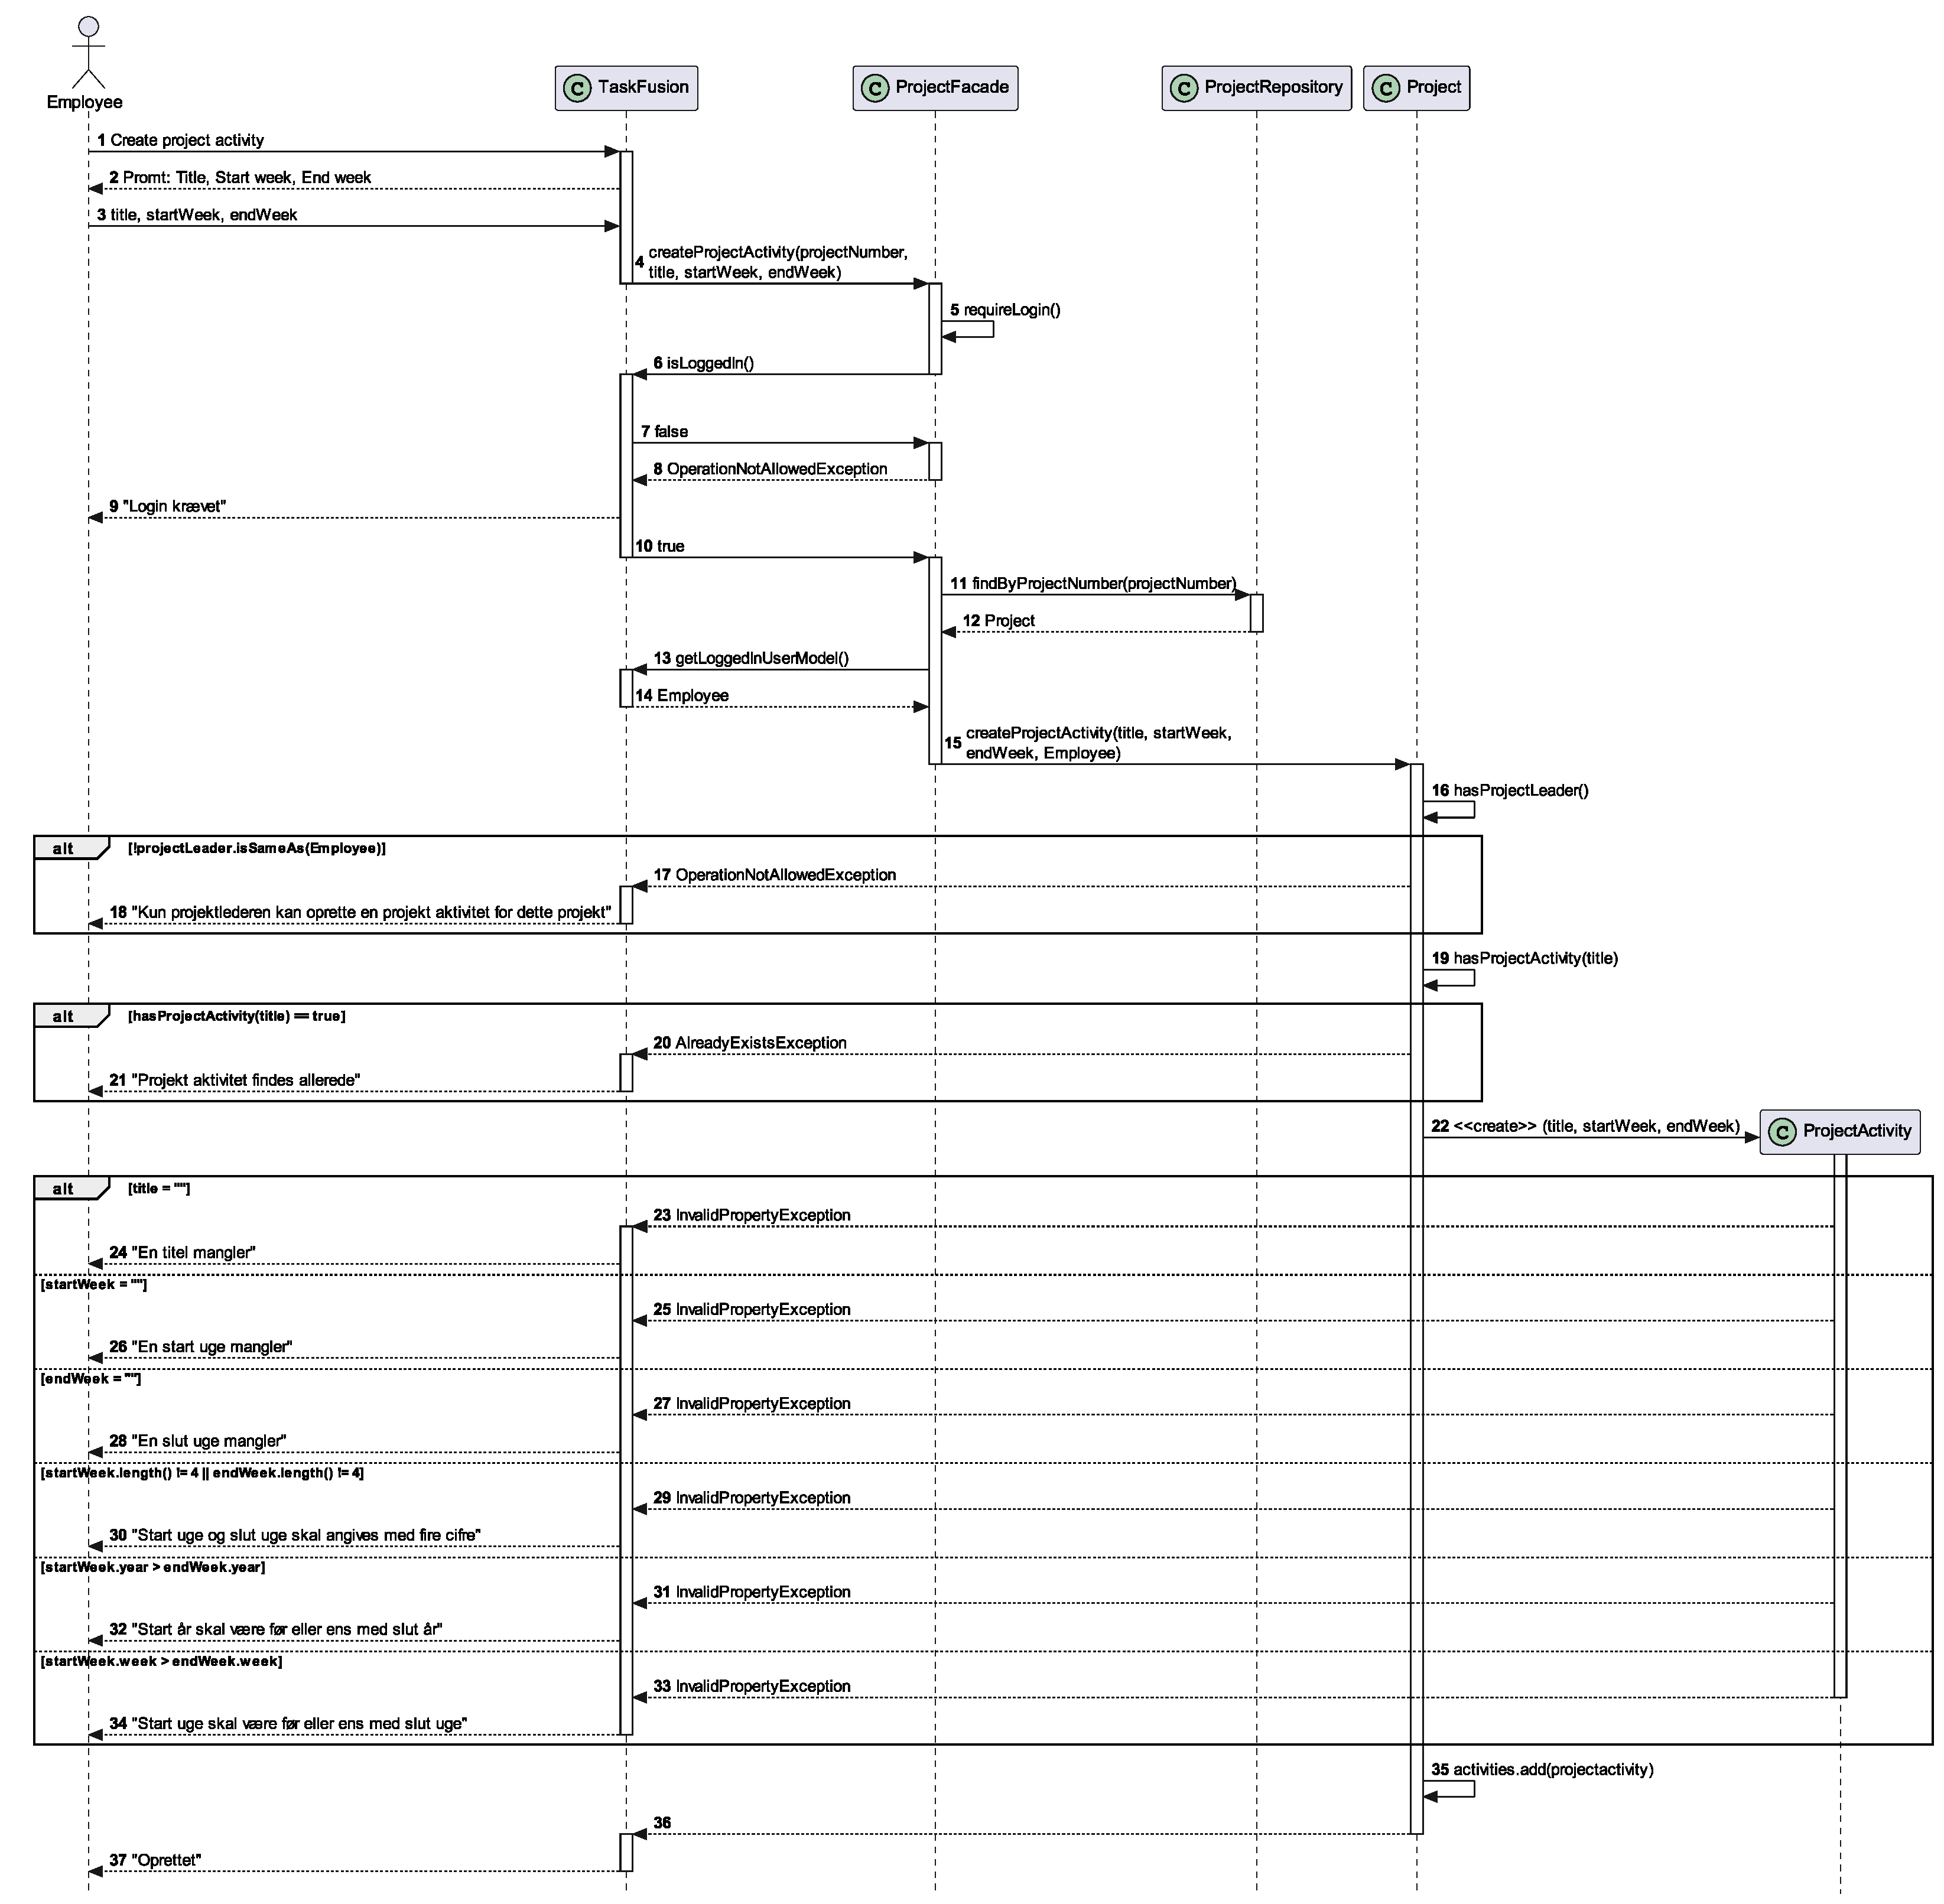
\includegraphics[width=.8\textwidth]{RequirementsAndDesign/SequenceDiagrams/seqCreateProjectActivity.eps}
\end{figure}
\begin{landscape}
    \section{Klassediagram over program laget}\label{apdx:classDiagram_full}
    \begin{figure}[H]
        \centering
        \caption{Klassediagram over program laget}
        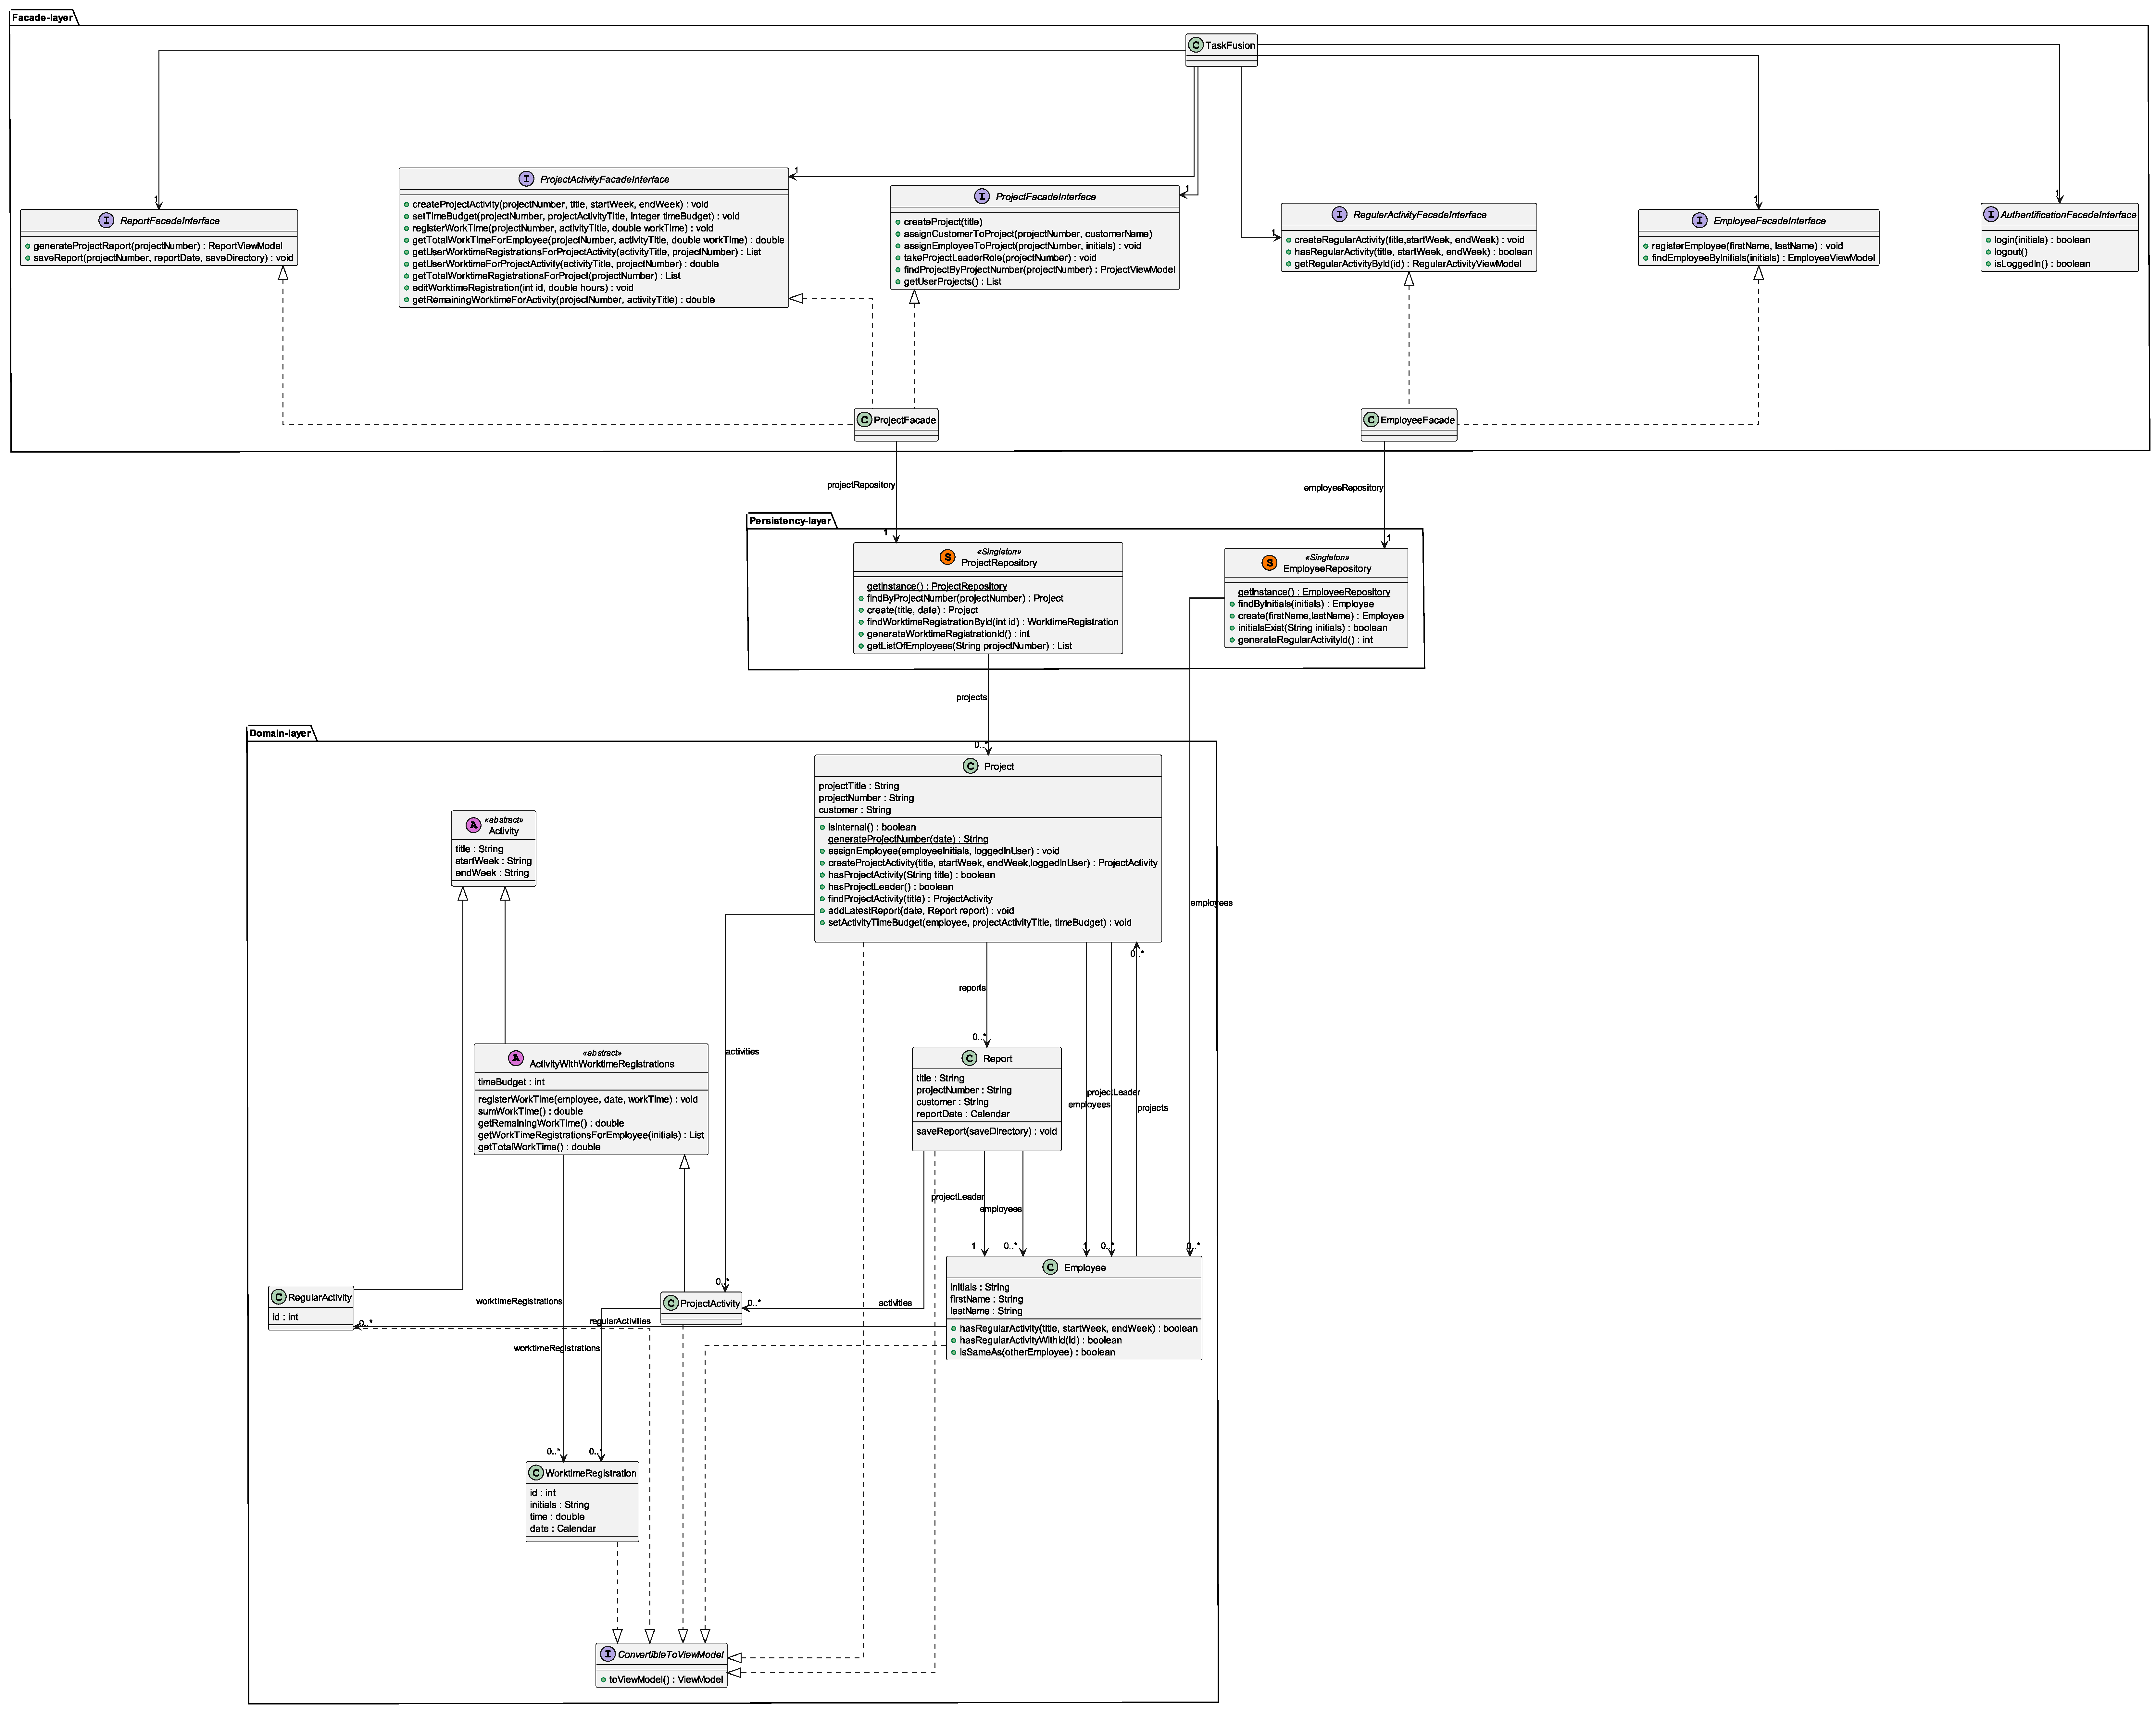
\includegraphics[width = \textheight]{ImplementationAndTest/Diagrams/ClassDiagrams/ClassDiagram_full.eps}
        \label{fig:classDiagram_full}
    \end{figure}
    \section{Klassediagram over præsentations-laget}\label{apdx:classDiagram_presentation}
    \begin{figure}[H]
        \centering
        \caption{Flowdiagram over CLI brugergrænsefladen}
        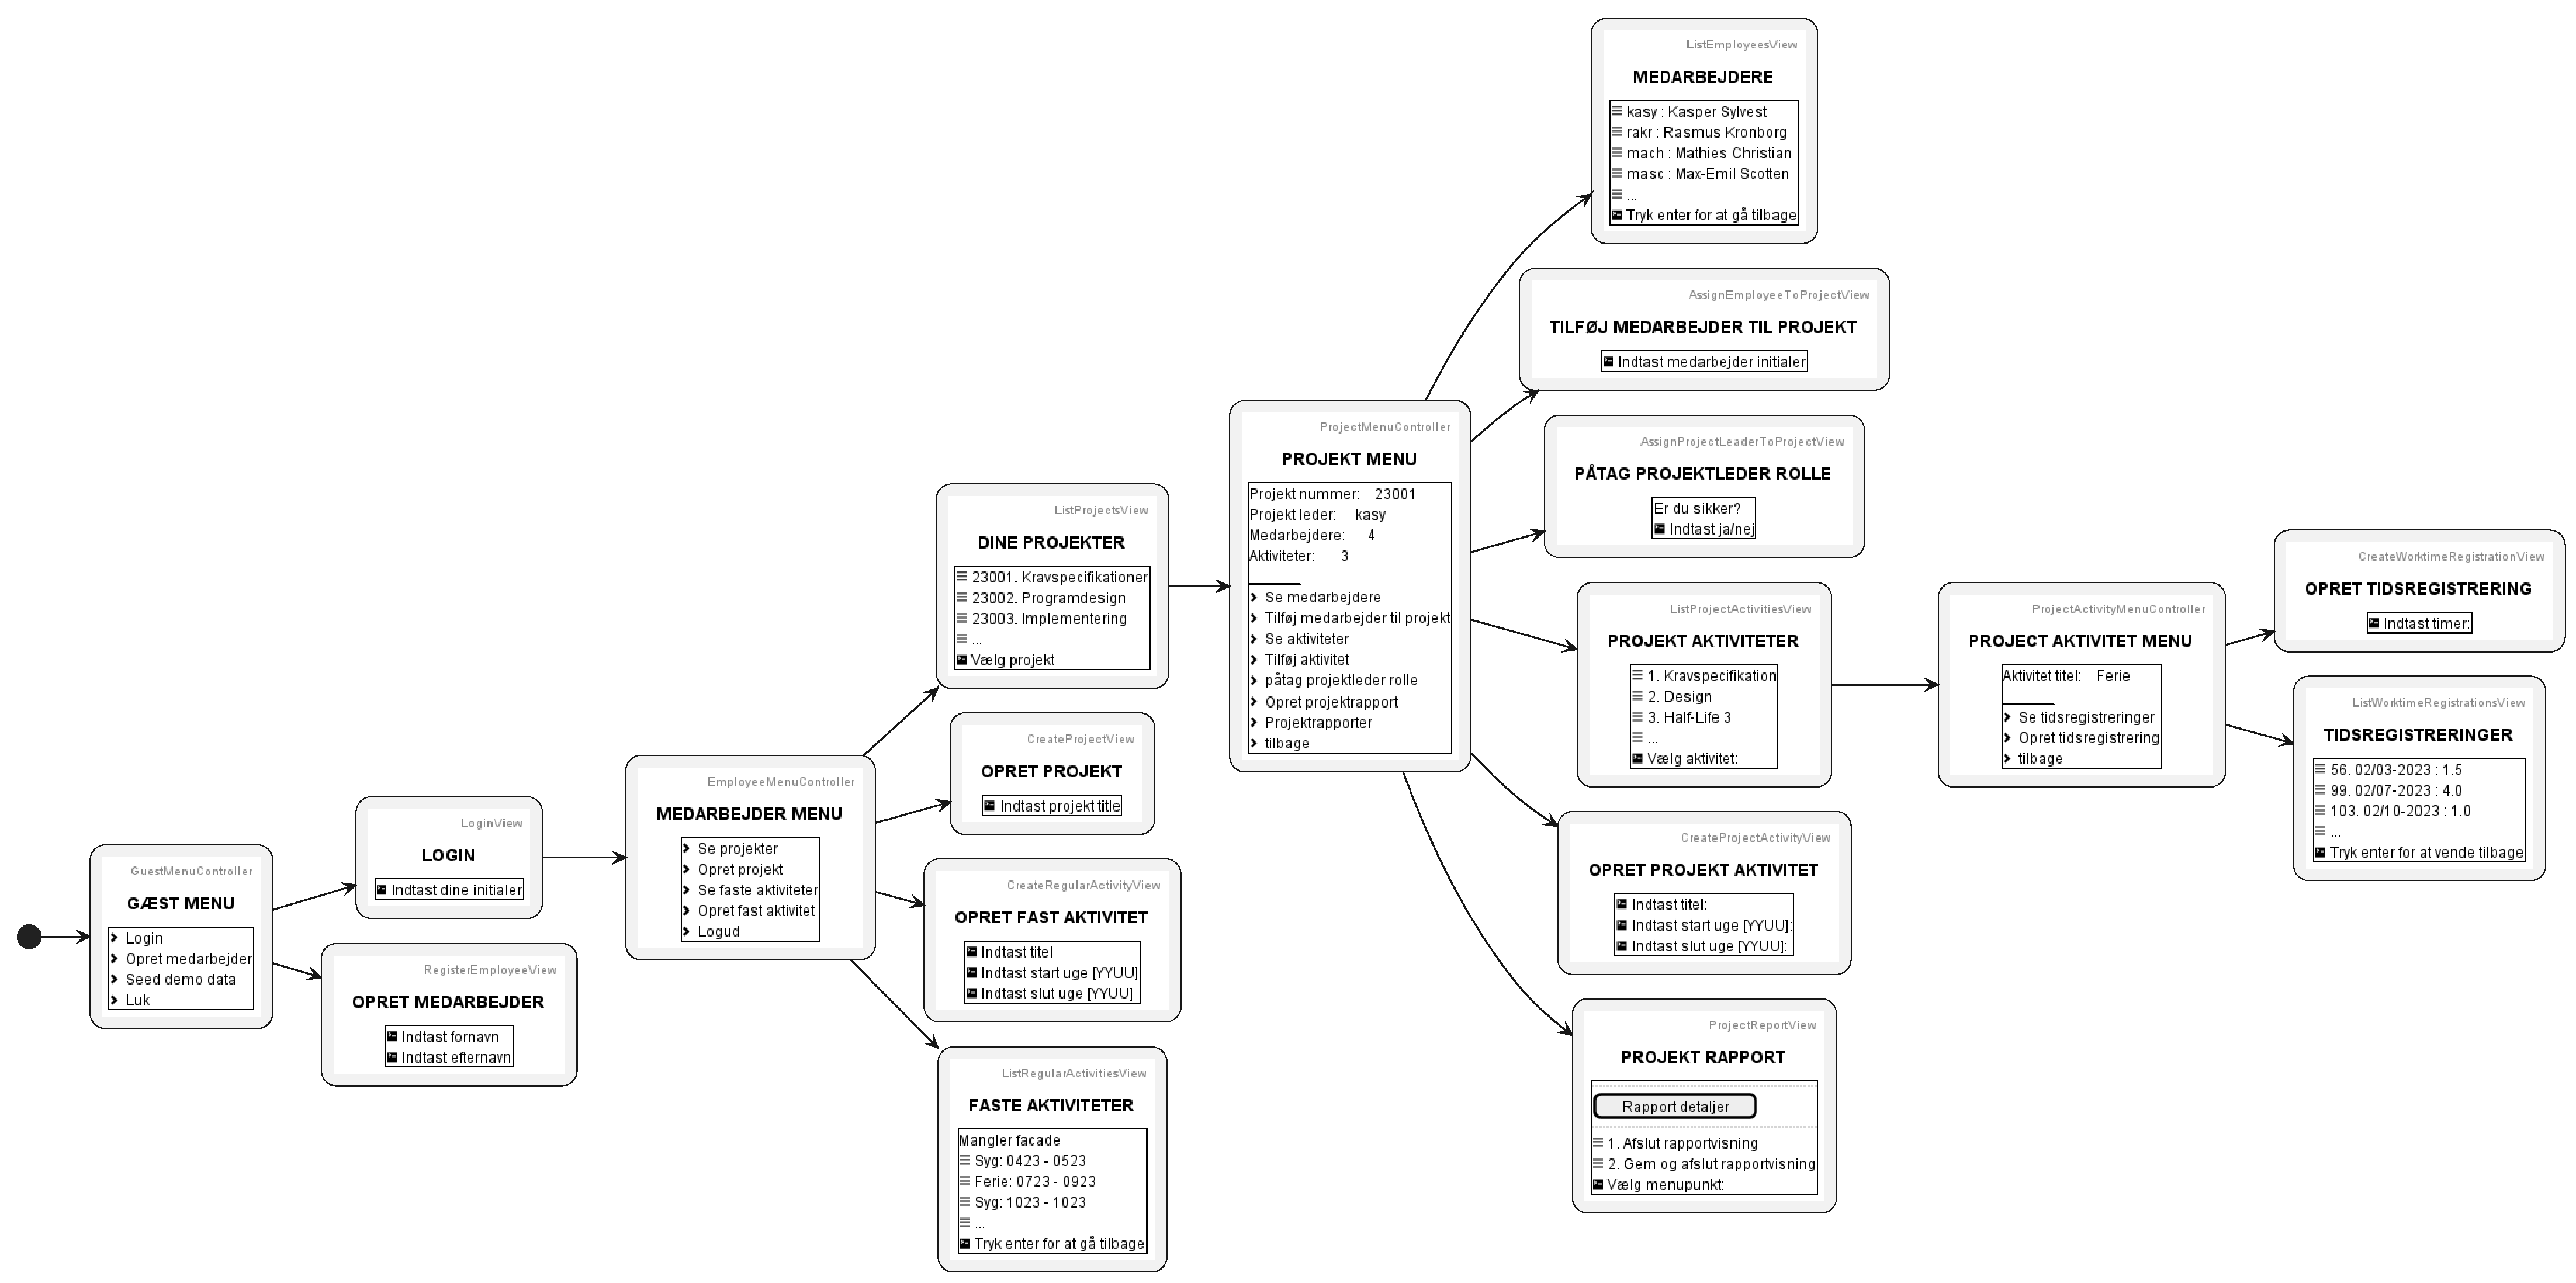
\includegraphics[width = \linewidth]{ImplementationAndTest/Diagrams/FlowCharts/flow_cli.eps}
        \label{fig:flow_cli_big}
    \end{figure}
    \section{Klassediagram over facade-laget}\label{apdx:classDiagram_facade_full}
    \begin{figure}[H]
        \centering
        \caption{Detaljeret klassediagram af facade-laget}
        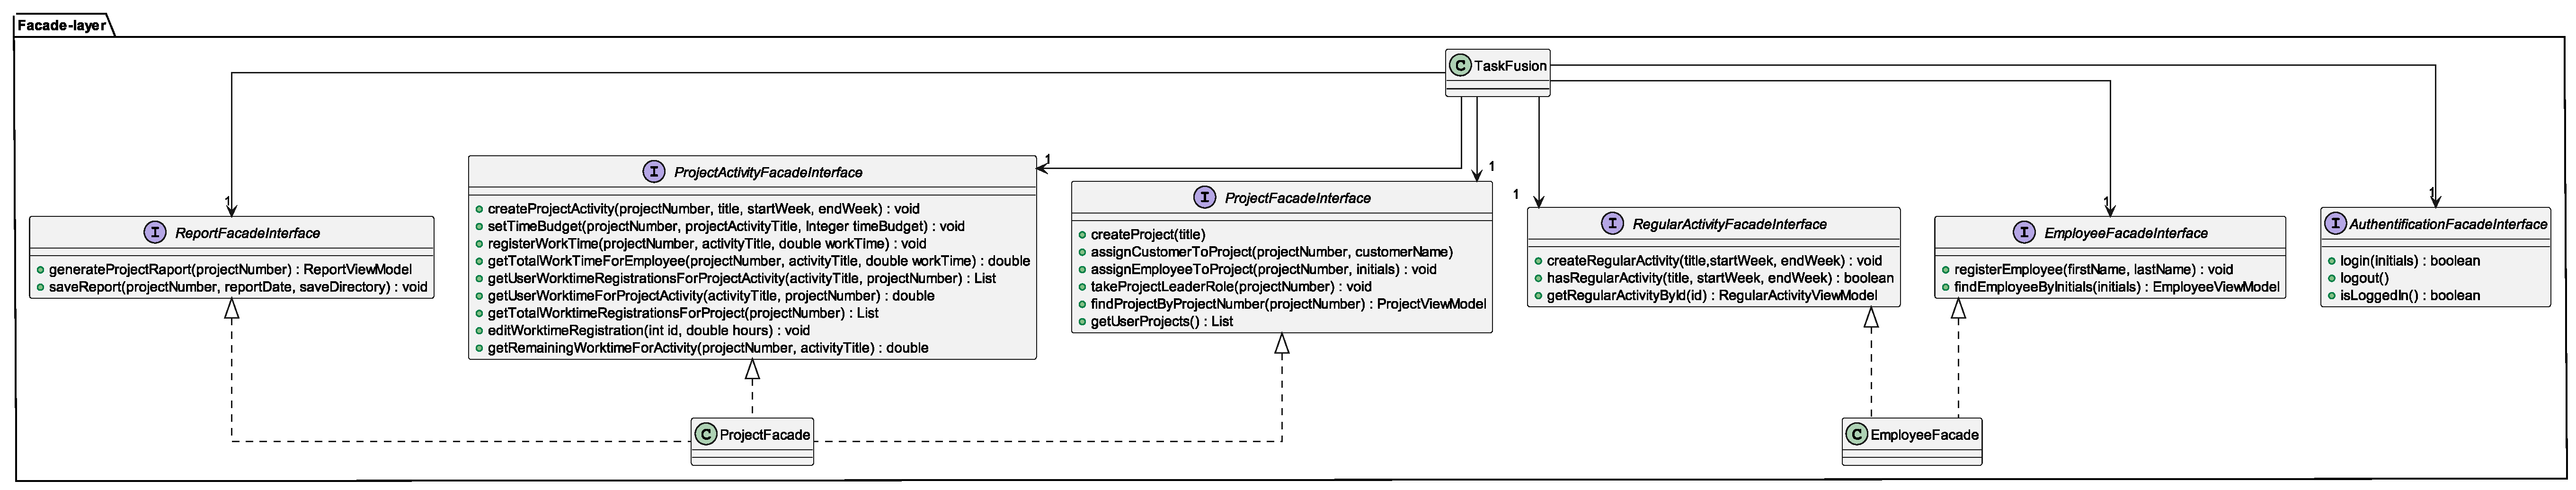
\includegraphics[width = \linewidth]{ImplementationAndTest/Diagrams/ClassDiagrams/ClassDiagram_facade_full.eps}
        \label{fig:class_facade_full}
    \end{figure}
\end{landscape}

\end{document}
